\chapter{Deployment Guide}


\section{Hardware Requirements}

CxAnalytix is recommended to run on a standalone server or as a Docker container. It can run on the CxSAST manager 
as it does not tend to have an extremely CPU intensive workload for most scan volumes. It is not recommended to run it on the CxSAST manager 
if it can be avoided.

\noindent\\
Basic runtime specification:
    \begin{itemize}
        \item 4GB RAM
        \item CPU Cores should be 1 more than the configured number of concurrent scan threads (i.e. \textit{number of threads} + 1)
        \item At least 1TB of space if storing extraction data for 2 weeks or less if you expect < 100 scans every 2 hours
    \end{itemize}


\section{MongoDB Sizing}

The MongoDB instance can be one of the following types of MongoDB:

\begin{itemize}
    \item Native MongoDB (local or cloud)
    \item AWS DocumentDB
\end{itemize}

\noindent Other types of MongoDB API compatible document databases may also work.  Azure's CosmoDB is currently not recommended at this time due to the 
maximum 2MB document size.  When CosmoDB officially supports the 16MB document size, it may be a viable option.

\noindent\\If persisting the extracted data in MongoDB, there is no set guide to sizing. Several variables should be considered in selection of system sizing.

\begin{itemize}
    \item Data Retention\\
    Most deployments intend to persist the vulnerability data in perpetuity (or don't have a plan to purge data). 
    If this is the case, a MongoDB cluster with the ability to expand storage should be considered. This storage expansion will likely need to consider 
    sharding configurations that can be done as part of the MongoDB server configuration or via embedding a shard key directly in the stored data. 
    The \nameref{ShardKeyCookbook} can assist with choosing an appropriate configuration.

    \item Shard Searching\\
    Most searches for vulnerability data may not be done such that a specific set of shards can limit the scope of where the query is executed. This may result
    in searches across all shards. The expected volume of queries that may result in multi-shard searches should be taken into account when specifying the 
    cluster members' hardware specifics. The machine specification will also need to account for CPU required for any indexing and data ingestion.
\end{itemize}

\section{Network Connectivity Requirements}

\subsection{SAST Connections Diagram}
Figure \ref{fig:SAST-network} shows the connection diagram for a CxAnalytix deployment. Where connections to REST APIs are indicated, the transport mechanism is 
HTTP/s over any port specified by the URL. Where connections to the SQL database are indicated, the connection is a regular socket using SQL server's wire protocol.

\noindent\\It is not recommended that the SQL server connection be exposed to the public internet. The SQL connection exists to support the audit log export capability 
and is not required to run CxAnalytix.\footnote{SQL connectivity is not available for Checkmarx hosted environments.}

\begin{figure}[h]
    \caption{SAST Network Connection Diagram}
    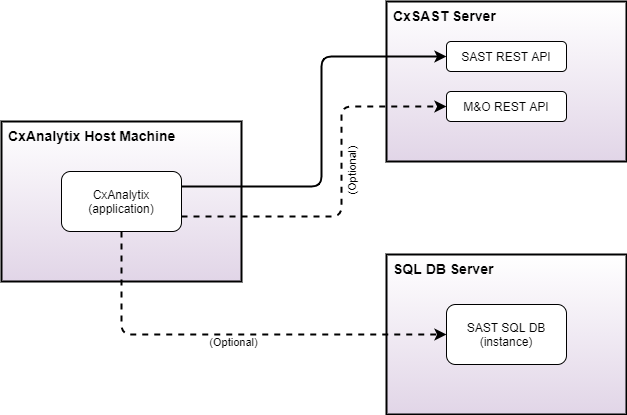
\includegraphics[width=\textwidth]{graphics/Deployment-SAST-connections.png}
    \label{fig:SAST-network}
\end{figure}

\subsection{Splunk Deployment Diagram}
Figure \ref{fig:SPLUNK-network} shows a typical deployment of CxAnalytix with the Splunk Universal Forwarder. In this deployment,
the Universal Forwarder is configured to read the CxAnalytix log output and forward the data to a remote Splunk instance. The vulnerability 
data log locations are configured in the Log4Net configuration.

\noindent\\The Splunk Universal Forwarder should be configured to tail the CxAnalytix output, which will forward to Splunk.

\begin{figure}[h]
    \caption{Splunk Network Connection Diagram}
    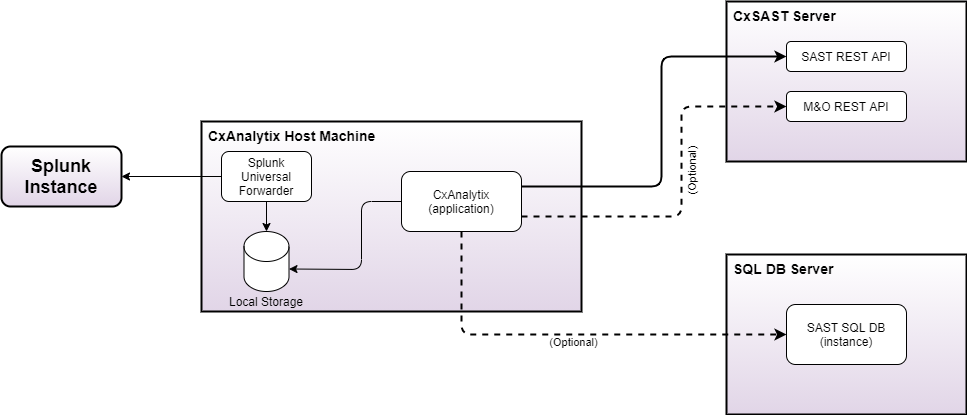
\includegraphics[width=\textwidth]{graphics/Deployment-SPLUNK-connections.png}
    \label{fig:SPLUNK-network}
\end{figure}


\subsection{MongoDB Deployment Diagram}
Figure \ref{fig:MONGO-network} shows a typical deployment of CxAnalytix configured to write vulnerability data to a MongoDB database. 
The MongoDB instance may be an on-premise instance or an instance hosted in the cloud.

\begin{figure}[h]
    \caption{MongoDB Network Connection Diagram}
    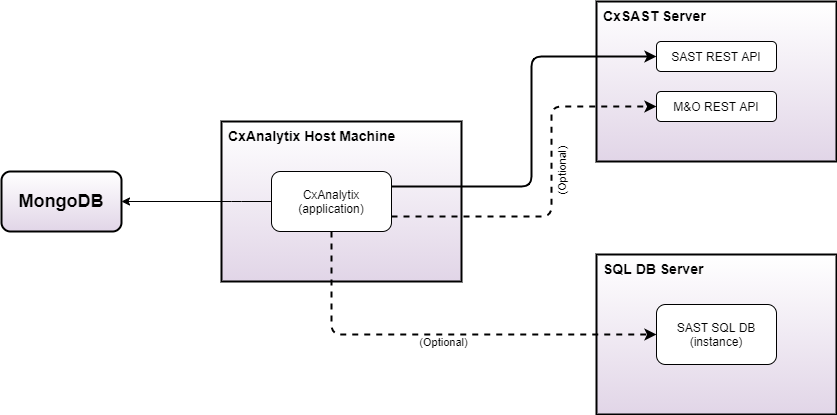
\includegraphics[width=\textwidth]{graphics/Deployment-MONGO-connections.png}
    \label{fig:MONGO-network}
\end{figure}


\section{Configuration Backups}
The crawl state storage files should be archived periodically to ensure crawling does not re-crawl existing scans. The state files are written to the path 
specified by the \verb|StateDataStoragePath| attribute in the \verb|CxAnalytixService| configuration section.  All files written to this path should
be archived periodically.

\noindent\\If running CxAnalytix as a Docker container, the default location \verb|/var/cxanalytix| should be mapped to a volume so that the state files are persistent across 
Docker container executions.  

\noindent\\The \verb|cxanalytix.config| file may also contain configurations that would be difficult to recreate.  It is advised that the configuration file be archived
after each change.

\section{Application Service Account}

An application service account is required for each service that CxAnalytix is configured to crawl.  If there are log messages indicating 
\verb|403: Forbidden| service API methods, this usually indicates the CxAnalytix role does not have appropriate privileges for that service.


\subsection{SAST}
CxAnalytix requires a SAST service account to authenticate with the SAST APIs to crawl scans. The service account has the following requirements:

\begin{itemize}
    \item The service account should be assigned at a team level that allows visibility to all projects that require crawling. 
    Usually this is the \verb|/CxServer|
    team but will depend on your configured team heirarchy. Any projects assigned to teams above or at a sibling level of the service account's assigned team 
    will not be visible to crawling requests.

    \item A role named CxAnalytix should be created and assigned to the service account user. The role should have the following minimum permissions:
    \begin{itemize}
        \item SAST->Project \& Scans->Save Sast Scan
        \item Reports->Generate Scan Reports
    \end{itemize}

\end{itemize}

\subsection{SCA}

CxAnalytix requires an SCA service account authenticate with the SCA APIs to crawl scan reports. The service account has the following requirements:

\begin{itemize}
    \item The service account should be assigned at a team level that allows visibility to all projects that require crawling. 
    Usually this is the \verb|/CxServer|
    team but will depend on your configured team heirarchy. Any projects assigned to teams above or at a sibling level of the service account's assigned team 
    will not be visible to crawling requests.

    \item A role named CxAnalytix should be created and assigned to the service account user. The role should have the following minimum permissions:
    \begin{itemize}
        \item SCA Viewer
    \end{itemize}

\end{itemize}

